\section{Learning agents}\label{AI: Agent Programs/Learning agents}

\begin{figure}[H]
    \centering
    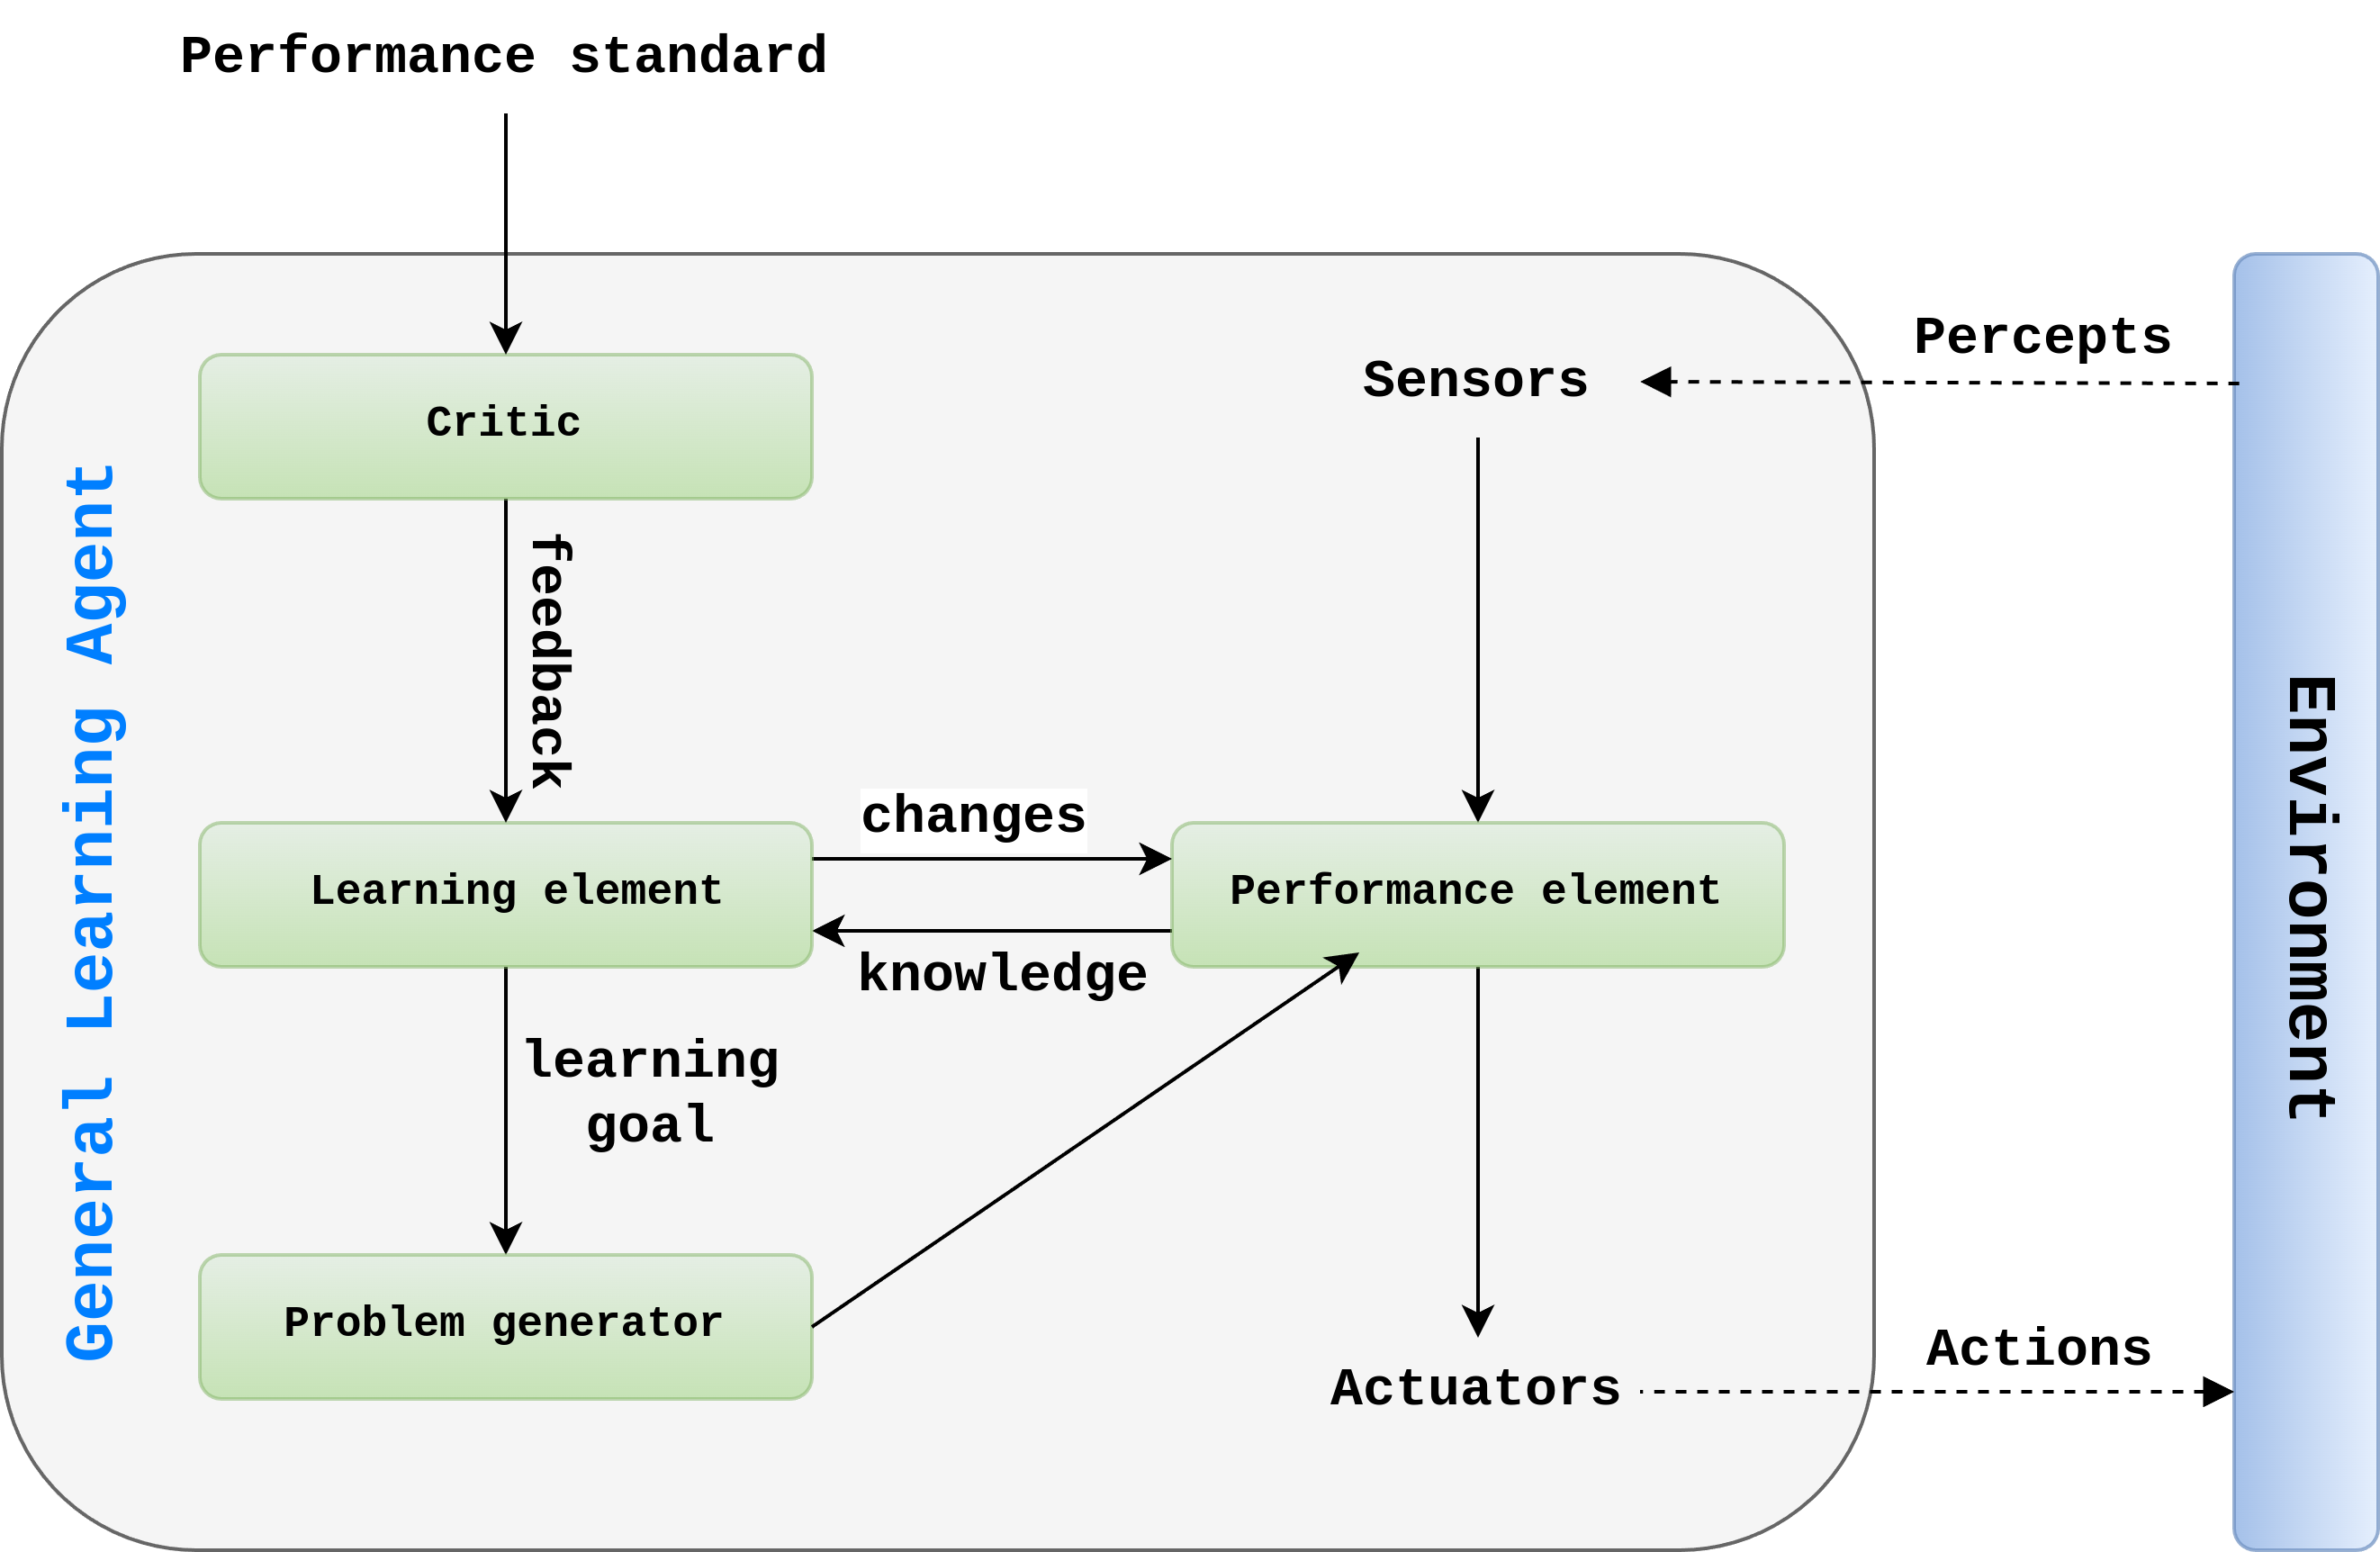
\includegraphics[
        width=0.5\linewidth, 
        height=6cm, 
        keepaspectratio
    ]{images/artificial-intelligence/ai-agents/agents-general-learning-agent.png}
    \caption*{A general learning agent. \cite{common/online/tools/draw.io}}
\end{figure}


\vspace{0.5cm}


\begin{enumerate}[itemsep=0.2cm]
    \item In his famous early paper, \textbf{Turing} (1950) considers the idea of actually programming his intelligent machines by hand.
    \hfill \cite{ai/book/Artificial-Intelligence-A-Modern-Approach/Russell-Norvig}

    \item  \textbf{advantage}: it allows the agent to operate in initially unknown environments and to become more competent than its initial knowledge alone might allow.
    \hfill \cite{ai/book/Artificial-Intelligence-A-Modern-Approach/Russell-Norvig}

    \item \textbf{conceptual components}:
    \begin{enumerate}[itemsep=0.1cm]
        \item \textbf{learning element}: responsible for making improvements
        \hfill \cite{ai/book/Artificial-Intelligence-A-Modern-Approach/Russell-Norvig}

        \item \textbf{performance element}: responsible for selecting external actions. it takes in percepts and decides on actions.
        \hfill \cite{ai/book/Artificial-Intelligence-A-Modern-Approach/Russell-Norvig}
        \\
        The design of the learning element depends very much on the design of the performance element. When trying to design an agent that learns a certain capability, the first question is \textbf{not} “\textit{How am I going to get it to learn this?}” \textbf{but} “\textit{What kind of performance element will my agent need to do this once it has learned how?}”
        \hfill \cite{ai/book/Artificial-Intelligence-A-Modern-Approach/Russell-Norvig}
        \\
        It is important that the performance standard be fixed. Conceptually, one should think of it as being outside the agent altogether because the agent \textbf{must not} modify it to fit its own behavior.
        \hfill \cite{ai/book/Artificial-Intelligence-A-Modern-Approach/Russell-Norvig}

        \item \textbf{critic}: The learning element uses feedback from the critic on how the agent is doing and determines how the performance element should be modified to do better in the future. 
        \hfill \cite{ai/book/Artificial-Intelligence-A-Modern-Approach/Russell-Norvig}
        \\
        The critic tells the learning element how well the agent is doing with respect to a fixed performance standard. The critic is necessary because the percepts themselves provide \textbf{no} indication of the agent’s success.
        \hfill \cite{ai/book/Artificial-Intelligence-A-Modern-Approach/Russell-Norvig}

        \item \textbf{problem generator}: It is responsible for suggesting actions that will lead to new and informative experiences. The point is that if the performance element had its way, it would keep doing the actions that are best, given what it knows. But if the agent is willing to explore a little and do some perhaps suboptimal actions in the short run, it might discover much better actions for the long run. 
        \hfill \cite{ai/book/Artificial-Intelligence-A-Modern-Approach/Russell-Norvig}
        \\
        The problem generator might identify certain areas of behavior in need of improvement and suggest experiments.
        \hfill \cite{ai/book/Artificial-Intelligence-A-Modern-Approach/Russell-Norvig}
         
    \end{enumerate}

    \item The learning element can make changes to any of the “\textit{knowledge}” components in the previous agents(simple reflex, model based, goal based, utility based). The simplest cases involve learning directly from the percept sequence. Observation of pairs of successive states of the environment can allow the agent to learn “How the world evolves,” and observation of the results of its actions can allow the agent to learn “What my actions do.”.
    The forms of learning do not need to access the external performance standard.
    \hfill \cite{ai/book/Artificial-Intelligence-A-Modern-Approach/Russell-Norvig}


    \item In a sense, the \textbf{external performance standard} is the \textit{universal} one of making predictions that agree with experiment.
    \hfill \cite{ai/book/Artificial-Intelligence-A-Modern-Approach/Russell-Norvig}

    \item  In a sense, the performance standard distinguishes part of the incoming percept as a \textbf{reward} (or \textbf{penalty}) that provides direct feedback on the quality of the agent’s behavior. Hard-wired performance standards such as pain and hunger in animals can be understood in this way.
    \hfill \cite{ai/book/Artificial-Intelligence-A-Modern-Approach/Russell-Norvig}

    \item Learning in intelligent agents can be summarized as a process of modification of each component of the agent to bring the components into closer agreement with the available feedback information, thereby improving the overall performance of the agent.
    \hfill \cite{ai/book/Artificial-Intelligence-A-Modern-Approach/Russell-Norvig}

    
\end{enumerate}


